\chapter{Задача о парковочных местах}

\section{Подход №1}

Существует $M$ парковочных мест.

В игре участвуют $N$ игроков, $N >> M$.

$\tilde N$ --- количество севших за руль

$(N - \tilde N)$ --- количество поехавших общественным транспортом.

Издержки игроков $c(x)$:
\begin{itemize}
 \item  $t$, если $\tilde N\le M$,
 \item  $T$, если $\tilde N>M$;
 \item  $\tau$, альтернативный маршрут,
 \item  $t<\tau<T$
\end{itemize}

$\tau$ — альтернативный маршрут.
Сравнить его с лотереей ${t,T}$.
$P(t)$ задается $\tilde N$: $P=\frac{M}{\tilde{N}}$ (or $1$, if $M \le \tilde N$).

\textbf{Чистое равновесие}: $\frac{M}{\tilde N}t+(1-\frac{M}{\tilde{N}})T\approx\tau$.


$\tilde{N}$ (количество севших за руль) : $\frac{M}{\tilde{N}}t+(1-\frac{M}{\tilde{N}})T\le\tau$.

${N-\tilde N}$ (кто едет транспортом) : $\frac{M}{(\tilde{N}+1)}t+(1-\frac{M}{\tilde{N}+1})T\ge\tau$.

$T-\tau = \frac{M}{\tilde{N}}(T-t)$

$\tilde{N}=[\frac{M(T-t)}{T-\tau}]$ — чистое равновесие. Но «так не бывает», ибо неясно, кто эти счастливчики.

$p$ — вероятность сесть за руль.

$Q$[тебе достанется место] такова, что $\tau = Qt+(1-Q)T \Rightarrow Q(T-t)=T-\tau$, $Q*=\frac{T-\tau}{T-t}$.

Но! $Q$ должно быть вычислено как функция от $p$!

$(1-p)^{N-1} + \\ (N-1)p(1-p)^{N-2} + \\ C_{N-1}^2 p^2(1-p)^{N-2} + ... + \\ C_{N-1}^{M-1}p^{M-1}(1-p)^{N-M} + \\ C_{N-1}^{M}p^M(1-p)^{N-M-1}(\frac{M}{M+1}) + \\ C_{N-1}^{M+1}p^{M+1}(1-p)^{N-M-2}(\frac{M}{M+2}) + \\ p^{N-1}\frac{M}{N} = \\ Q^*$

Решить как обратную функцию, найти $p^*$ — решение $p^*(\frac{T-\tau}{T-t})$.

\subsection{Гипотеза}
В равновесии $Np^* >> M$.

\subsection{Общее решение}

\setstretch{1}
\inputpython{../code/task1.py}{1}{41}

\subsection{Вариации}

Для $N=1000$:

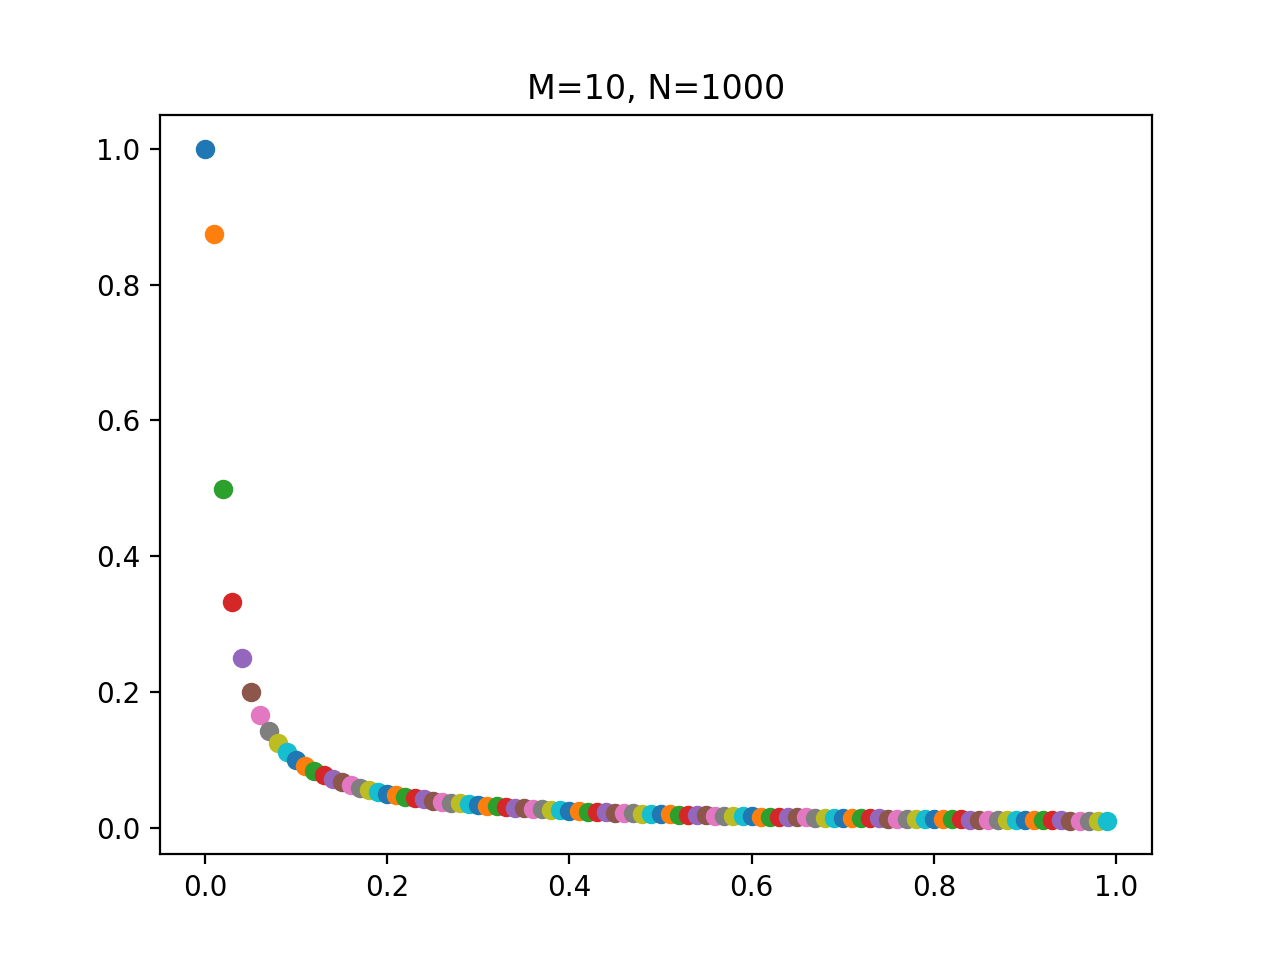
\includegraphics[scale=0.5]{img/1000_10}
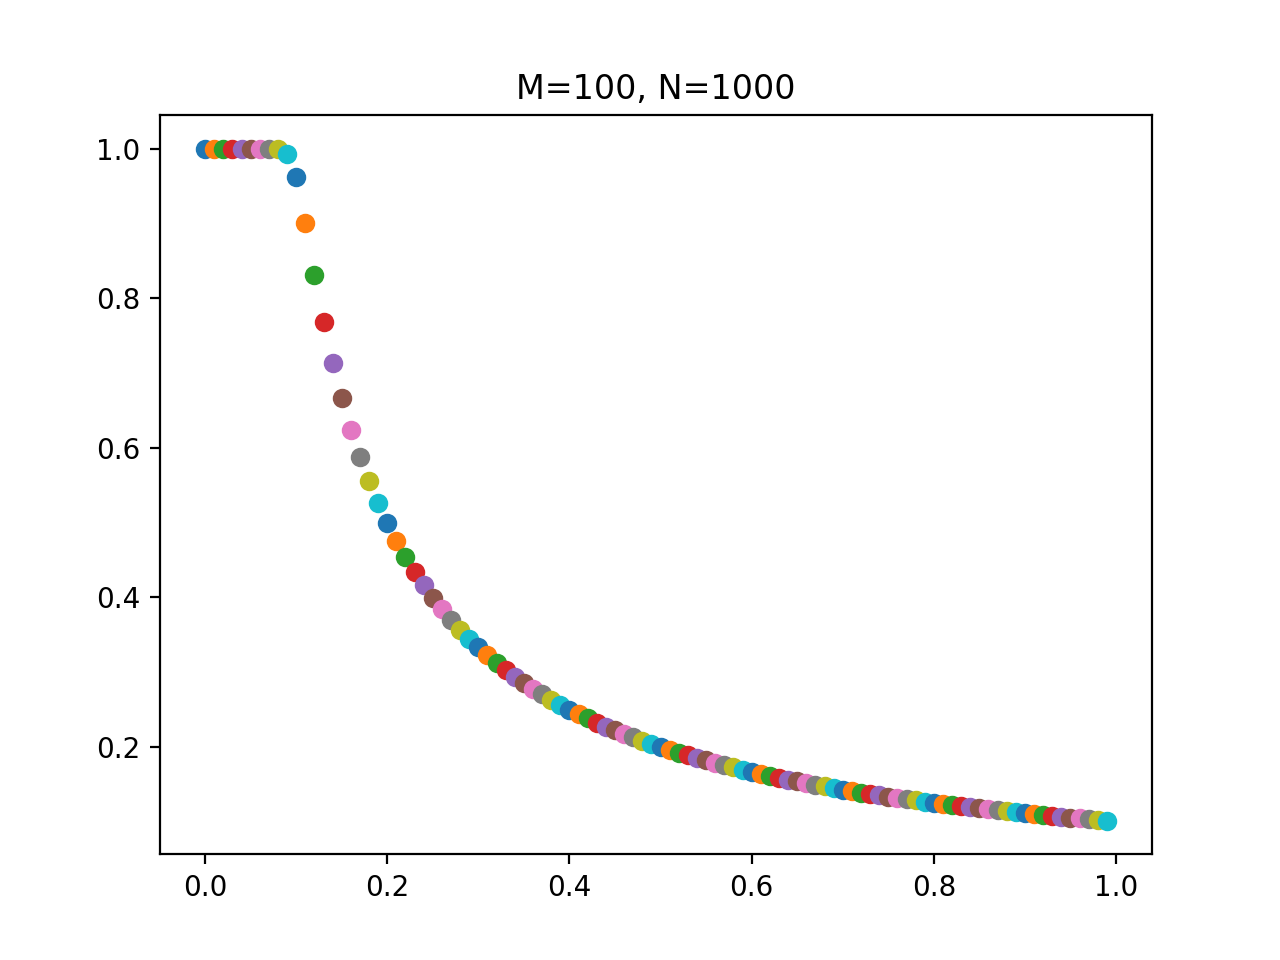
\includegraphics[scale=0.5]{img/1000_100}
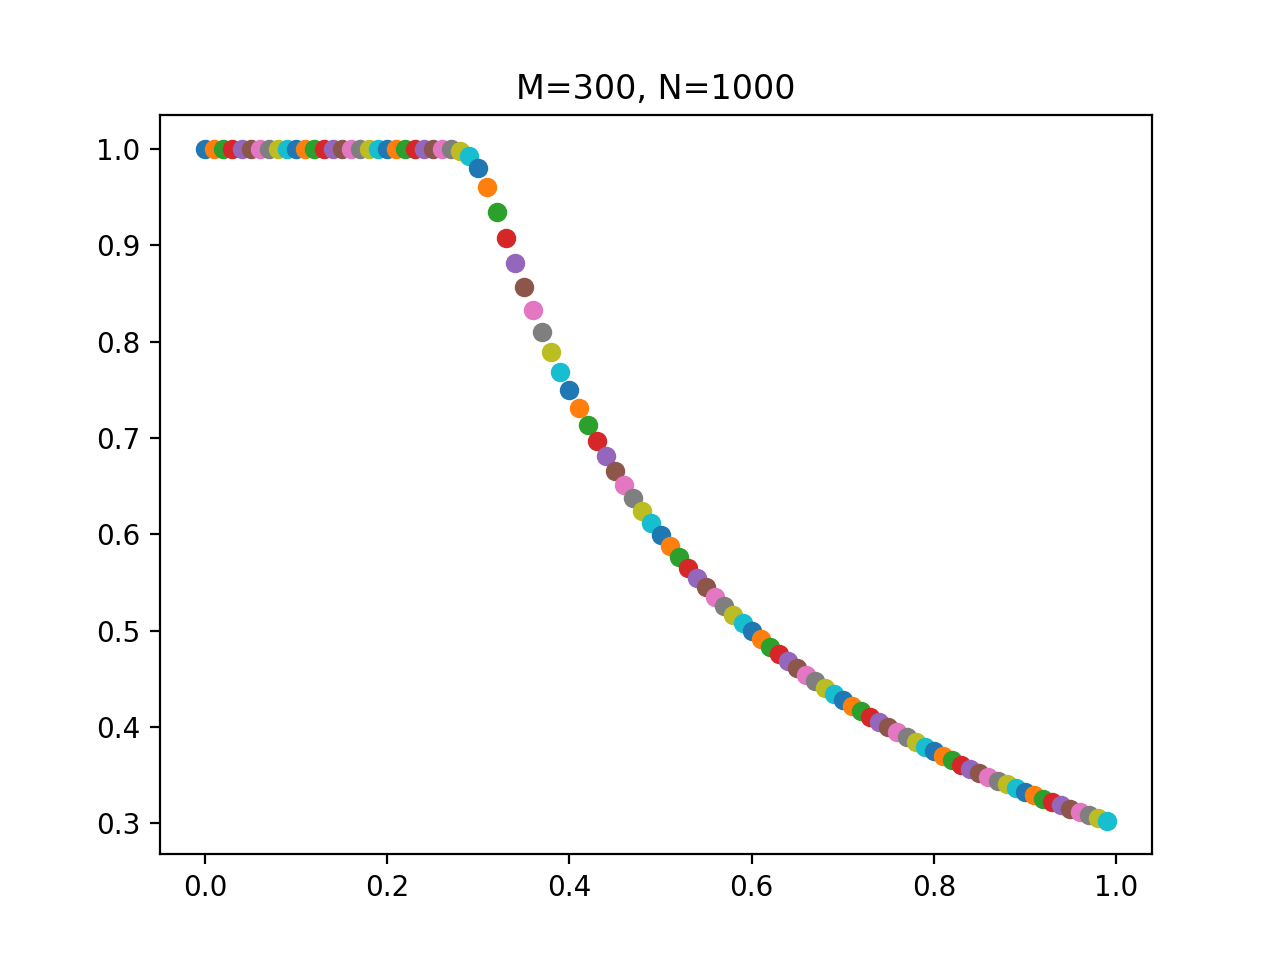
\includegraphics[scale=0.5]{img/1000_300}
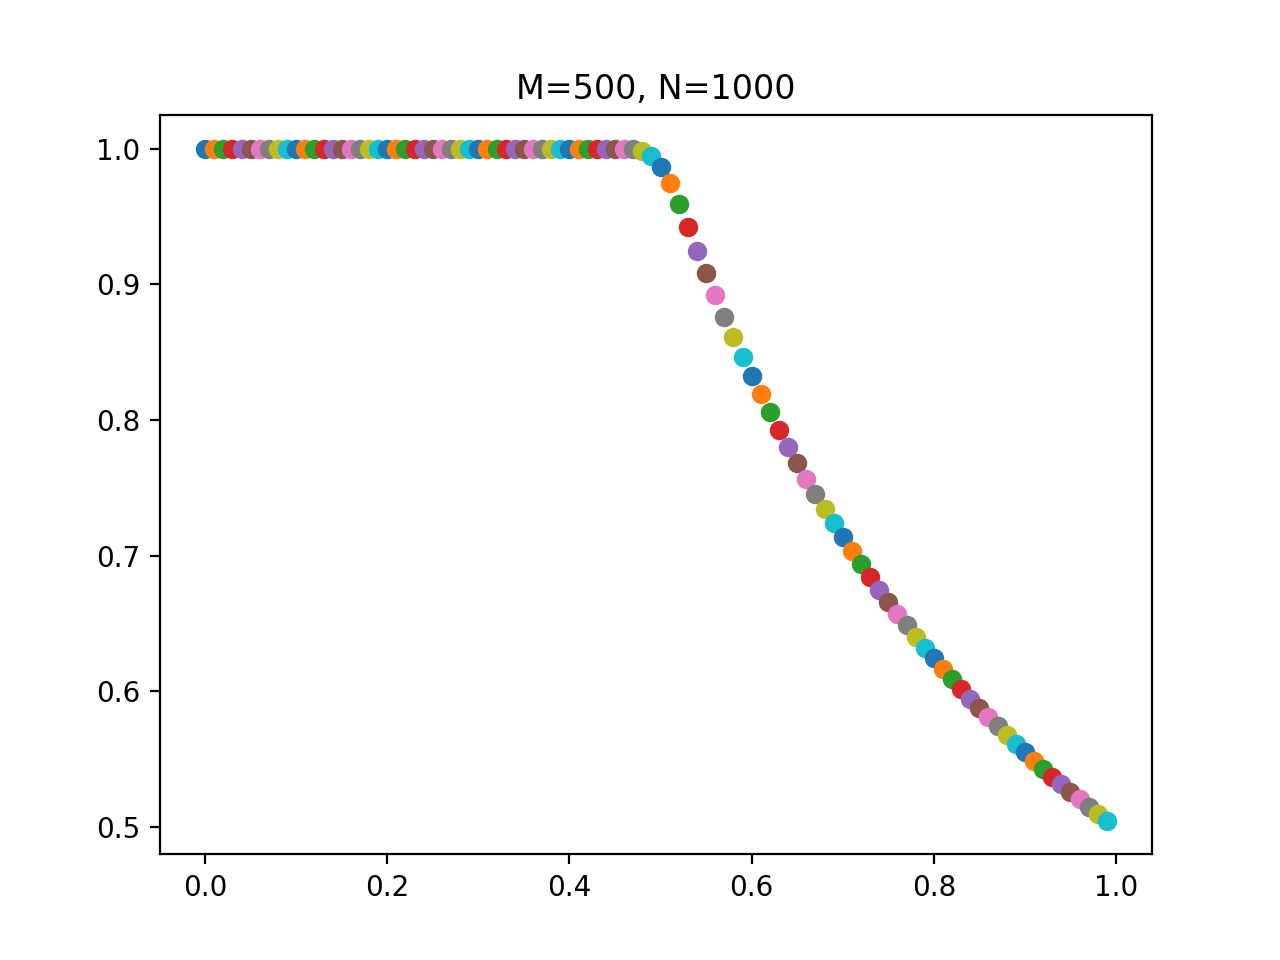
\includegraphics[scale=0.5]{img/1000_500}
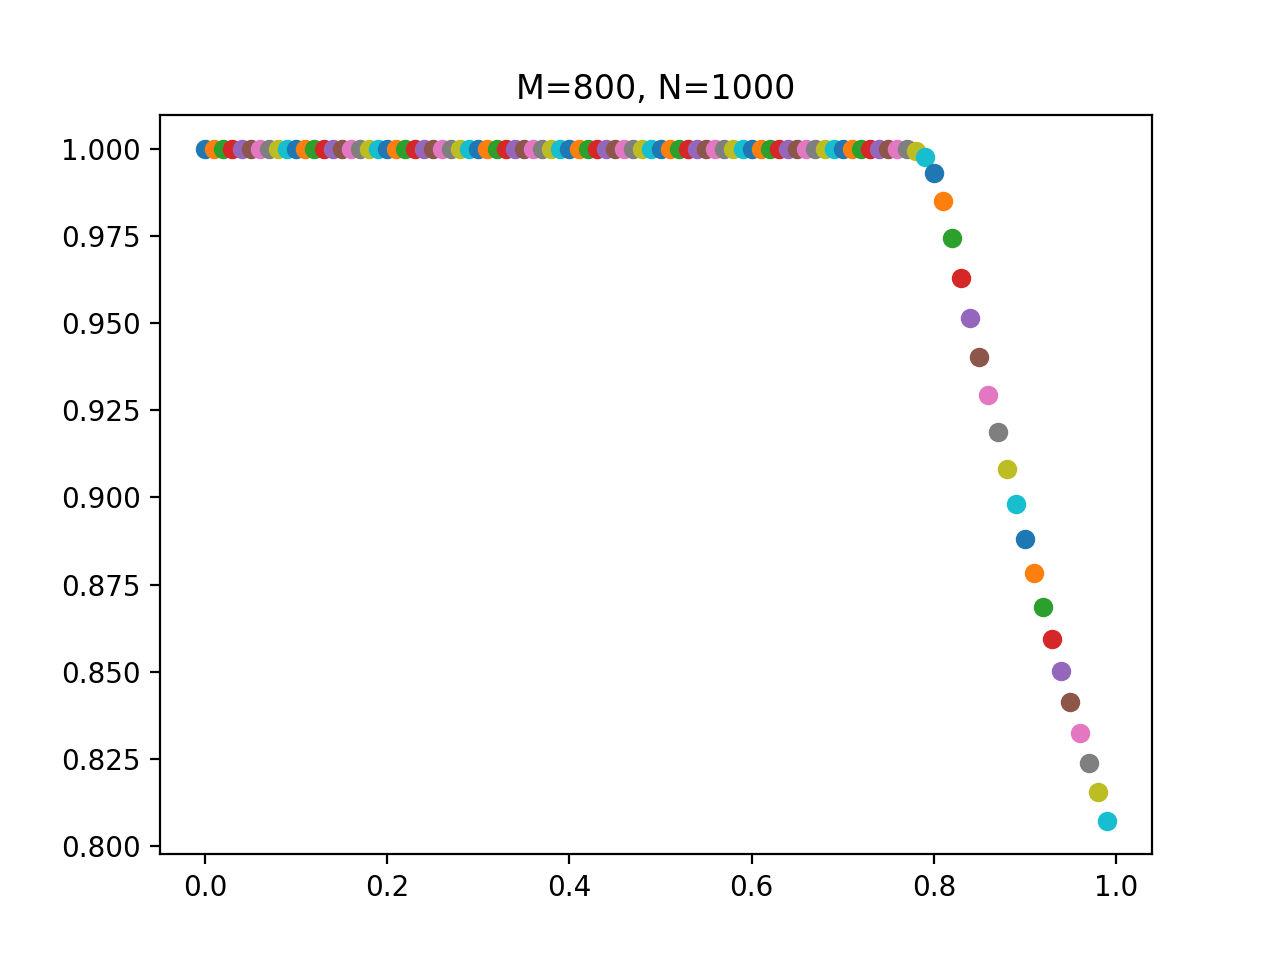
\includegraphics[scale=0.5]{img/1000_800}
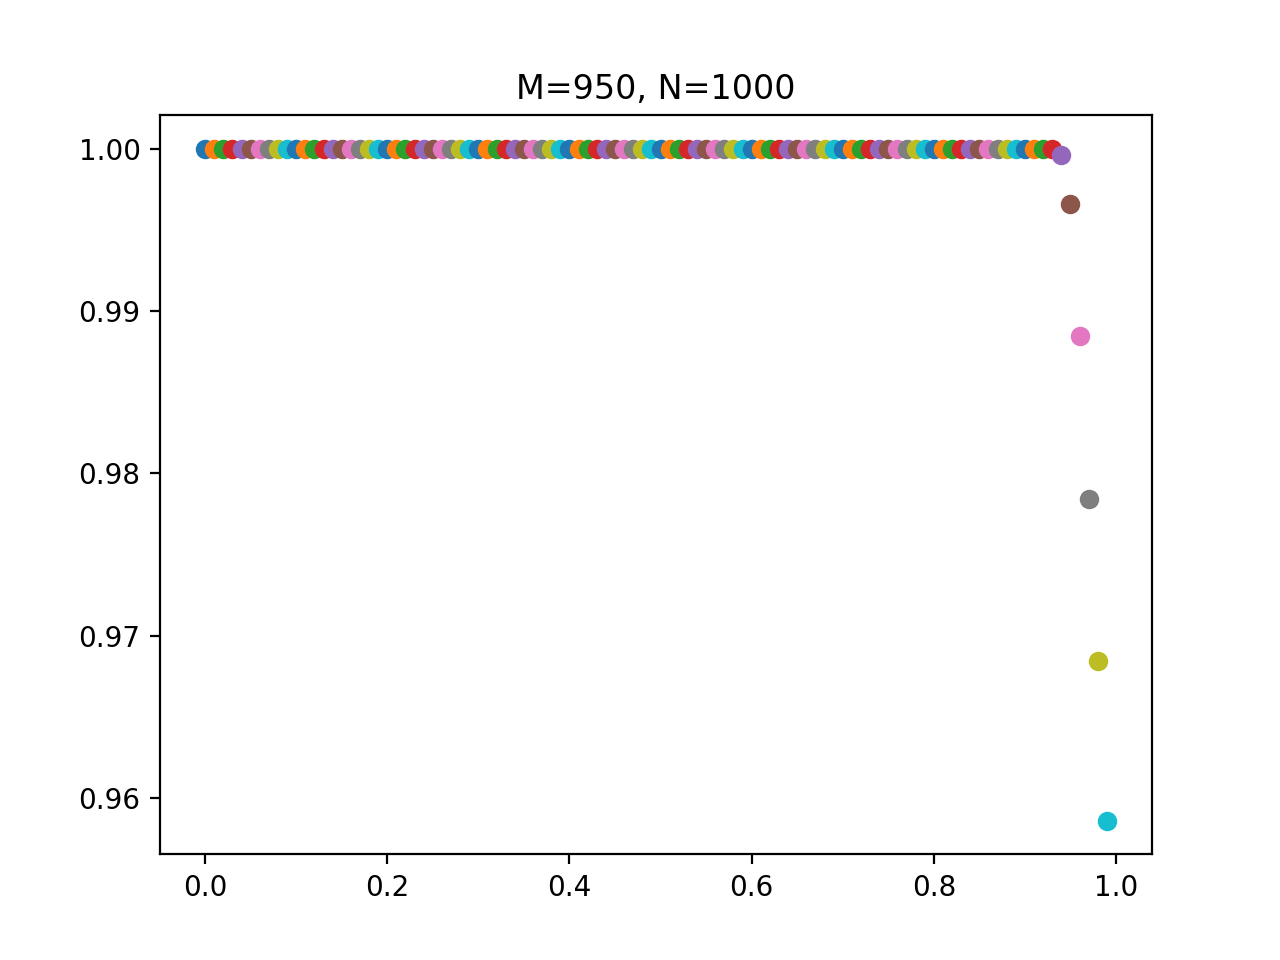
\includegraphics[scale=0.5]{img/1000_950}
\skip
Для $N=100$:

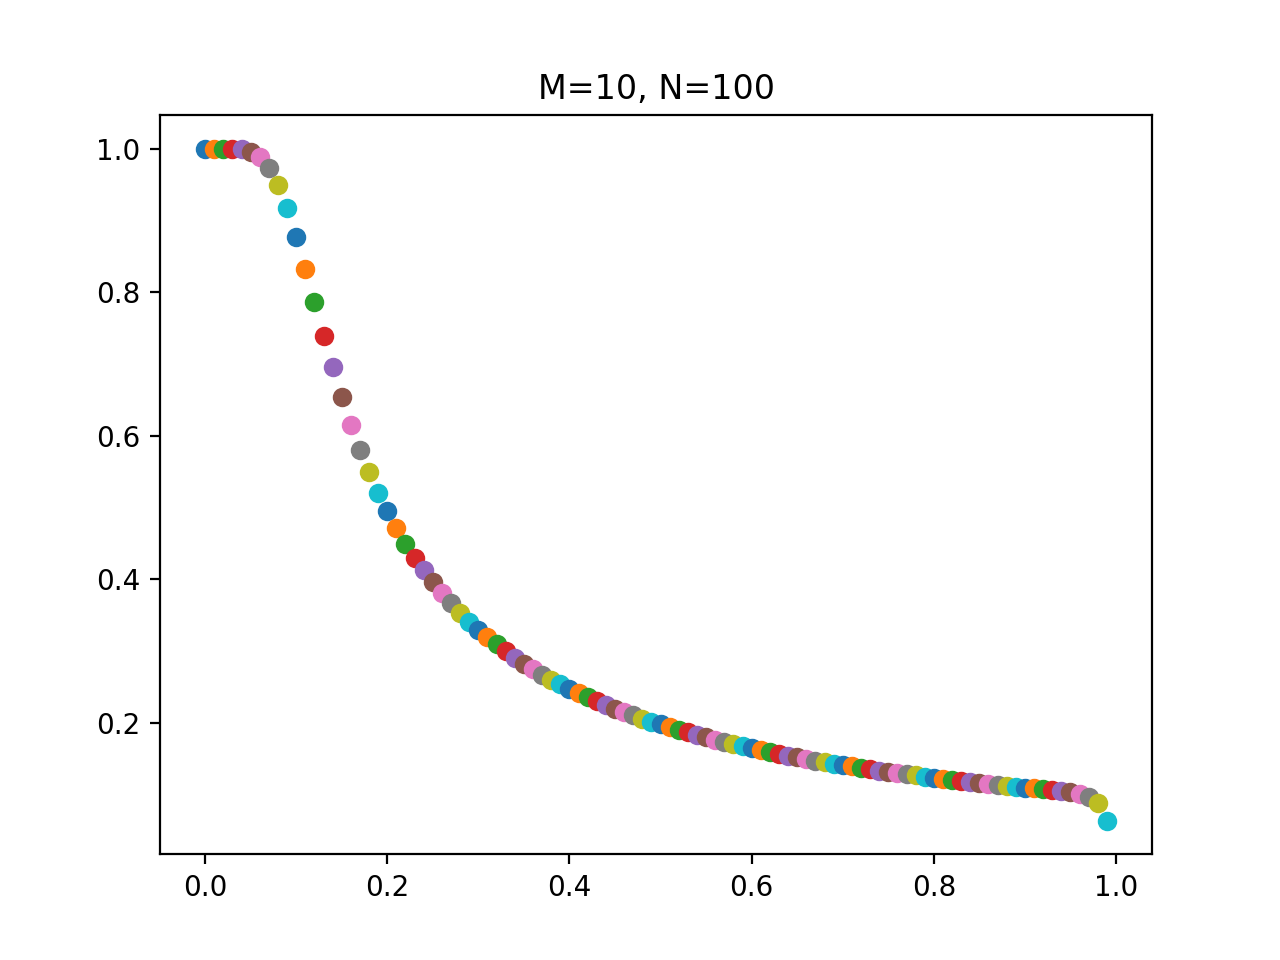
\includegraphics[scale=0.5]{img/100_10}
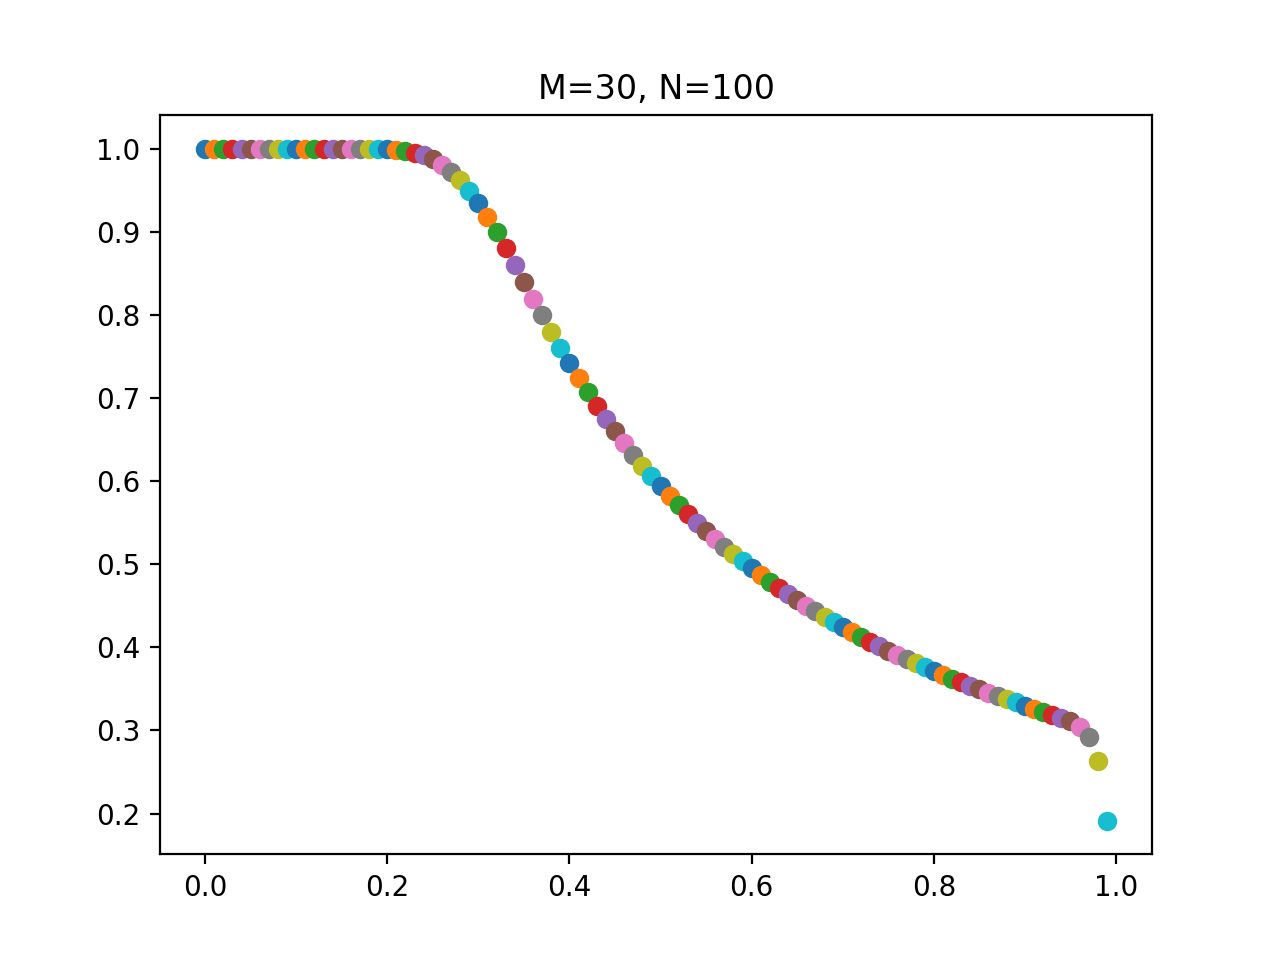
\includegraphics[scale=0.5]{img/100_30}
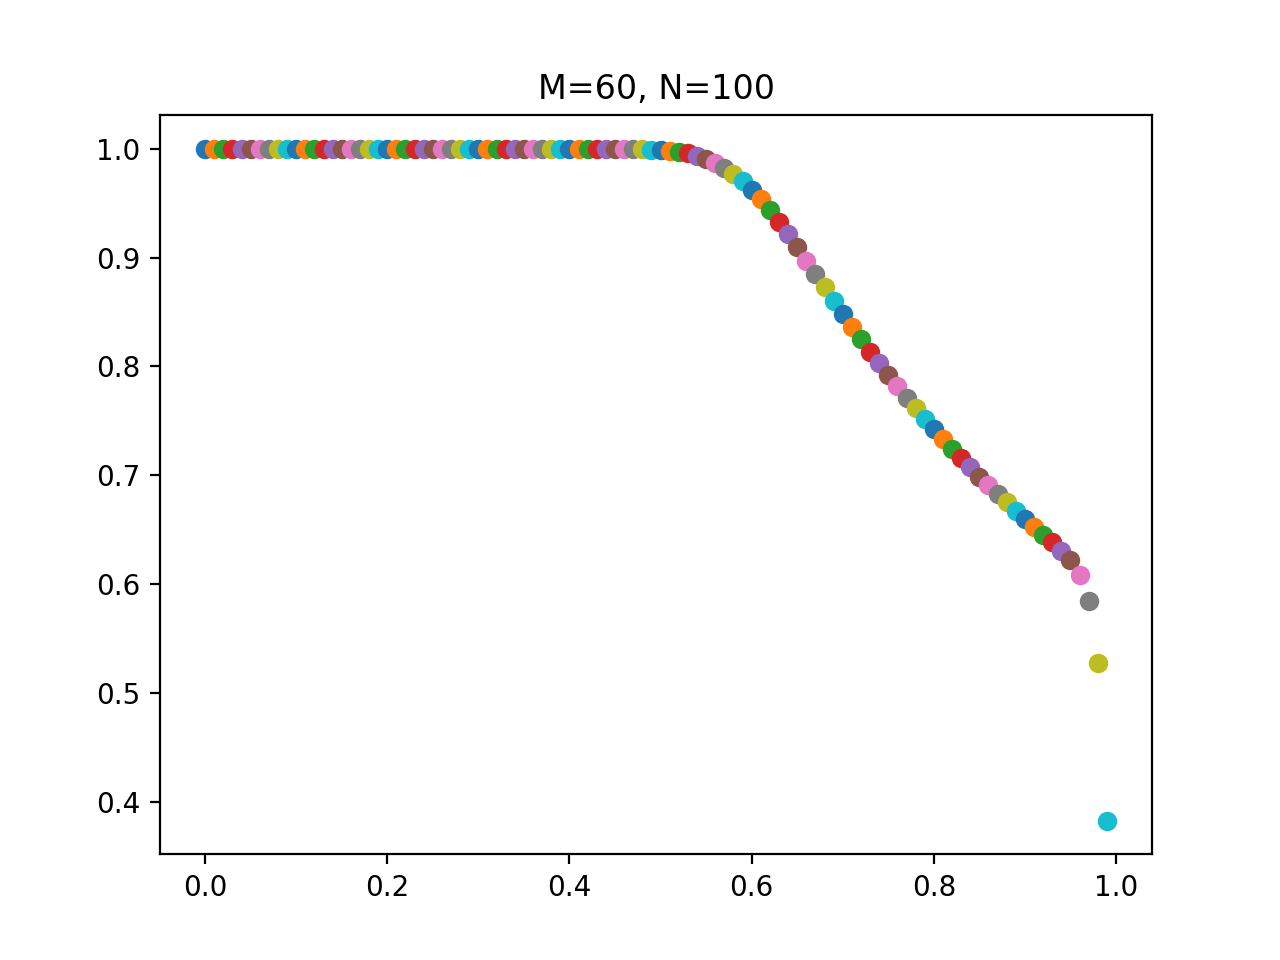
\includegraphics[scale=0.5]{img/100_60}
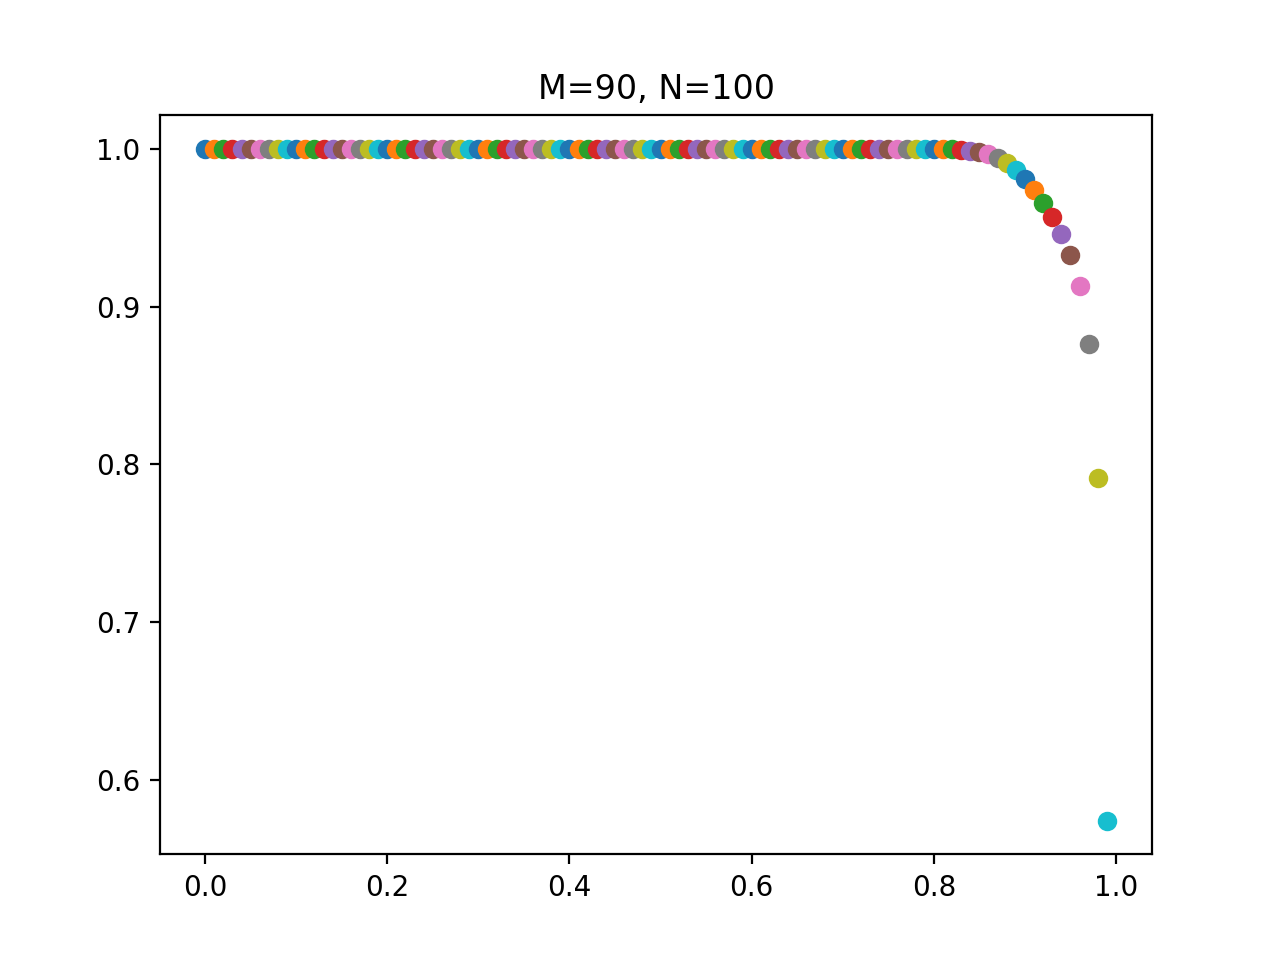
\includegraphics[scale=0.5]{img/100_90}



\section{Подход №2}

\setstretch{2}
% Это расшифровка записанного разговора

\subsection{Общая идея}

Когда M и N большие, задачу точно не нужно решать. И мы можем попробовать эту гипотезу, что не надо решать точно, проверить на таких M и N, на которых пока еще точно решается. При помощи программы решается при $M,N \le 1000$, но достаточно $M,N \le 100$. Это статфизическое приближение, которое будет простым и, скорее всего, в районе $100$ уже точным.

Если эта гипотеза верна, то для больших уже все делается приближенными вычислениями. И можно уже прилагать и проверять для примеров из раздела \ref{examples}.

Итак, есть три величины: 
\begin{itemize}
	\item $t$ --- если "повезло"
	\item $\tau$ --- если на общественном транспорте
	\item $T$ --- если попал в пробку
\end{itemize}

\begin{itemize}
	\item $M$ --- количество парковочных мест
	\item $N$ --- всего людей
\end{itemize}

Ситуация такова: мы ищем некоторое $p$ --- долю тех, кто едет (в равновесии).
Но на самом деле тогда в среднем поедет $pN$ в любом случае.
Если это большие величины, то будет очень больщая точность.
Тогда в среднем $\frac{M}{pN}$ будет вероятностью попадания, а $1 - \frac{M}{pN}$ --- непопадания (очень жесткое, грубое приближение).

И тогда получается формула $p = M/N * (T-t) / (T-\tau)$

И в равновесии отношение числа поехавших к числу парковочных мест не зависит ни от чего, кроме $T, \tau, t$: это просто $(T-t)/(T-\tau)$.

И эта гипотеза может быть проверена \textit{эмпирически}, если в данном конкретном городе разного размера стадионы дают примерно одинаковое отношение, то именно $T, \tau, t$ определяются городом, а $M$ и $N$ --- тонкости конкретных объектов проведения мероприятий.

То есть, если люди осведомлены о происходящем, то в среднем должно быть в каждом конкретном городе именно так. Это характеристика города: сколько раз происходит неудача
 % факап
 --- это первое интересное сообщение, которое можно сделать.
 % вывод, который будет очень броским

\subsection{Интересное продолжение}

$t$ и $\tau$ ни от чего не зависят.
А $T$ на самом деле зависит от $p$, и, соответственно, от величины $r= \frac{M}{pN}$.
Если много ищущих мест, то им сильно сложнее найти парковку, а если немного, то проще в соседних дворах.

% Можно протестировать какие-то очень просты формы
% Есть идея, что корень в некотором месте извлекается, потому что если территория вокруг увеличивается по квадрату, то поиск по корню. Время --- это время последующего приближения к центру после того, как ты нашел парковку
Соответственно, ключевой параметр, который нам нужен (мы его оцениваем) --- $\frac{M}{pN}$. Не само $p$, а именно выражение отношения количества парковочных мест к количеству поехавших. Это та переменная величина, которая нас и нтересует и которую мы ищем.

И в результате уравнений получается, что эта величина $r = T(r) -  \tau/(T-t)$
И теперь предполагаем, что $T = t + f(r)$, где $f(r)$ начинается с нуля при $r = 1$, а потом она растет вверх влево к бесконечности. И получается, что некоторая константа "мировая", равная $\tau - t$ --- разница между потраченным временем в транспорте и на своей машине, если ты попал сразу на парковку, приравнивается $(1-r)*f(r)$. Решение такого уравнение и есть равновесие и нужная нам величина (в равновесии эта величина будет определяться таким уравнением).

Где-то будет корень: судя по всему, она аккуратно и четко убывает от бесконечности к нулю, и где-то она пересекает в одном месте эту кривую, и дальше вопрос в \texiti{функциональной форме} $f(r)$. $f(r)$ измеряется в минутах --- это потерянные дополнительные минуты в тех же единицах, в которы измеряются $t$ и $\tau$.

Параметром является $M/N$ (вместимость парковки на вместимость зала), и $f$ будет функцией от него, соответственно, решением этого уравнения.

% Конец расшифровки записи

\subsection{Уравнения}
% Расшифровка листочка со скриншота
%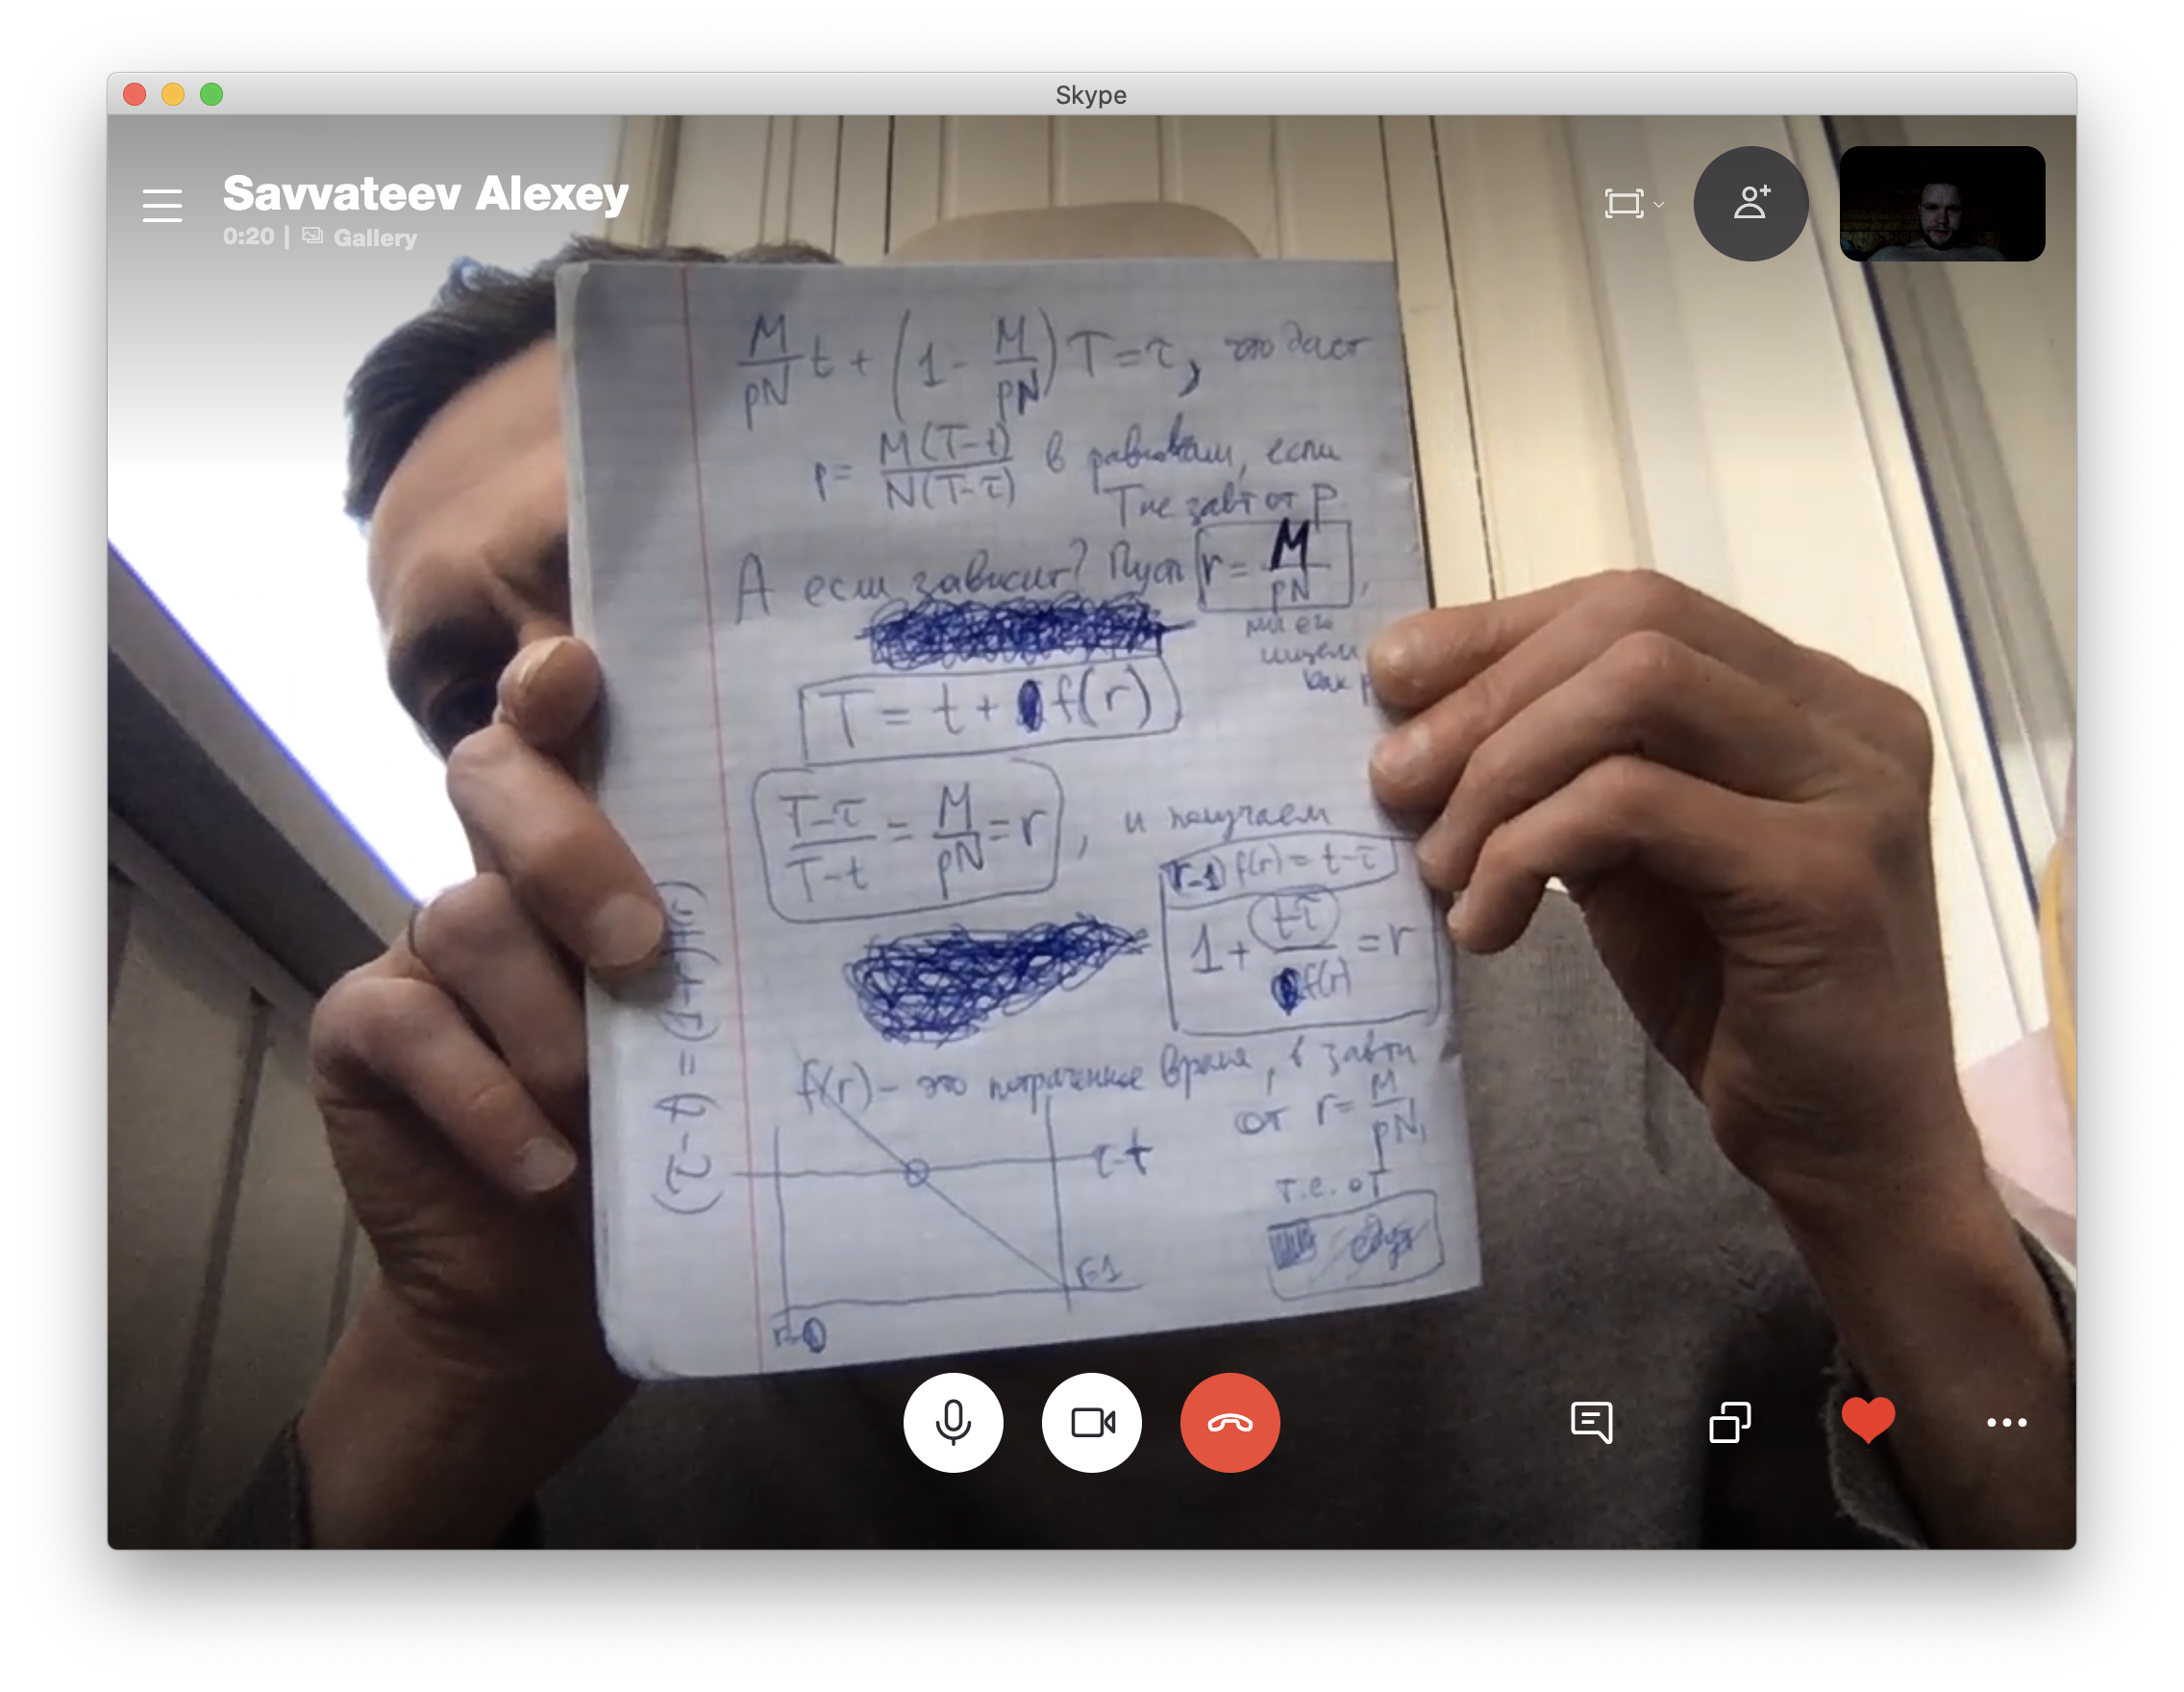
\includegraphics[scale=0.4]{img/tetrad2}
%(Этот скриншот временно вместо графика)

$\frac{M}{pN} t + (1 - \frac{M}{pN}) T = \tau$,
что дает
$p=\frac{M(T-t)}{N(T-\tau)}$ в равновесии, если $T$ не зависит от $p$.

А если зависит? Пусть $r = \frac{M}{pN}$

$T = t + f(r)$

$\frac{T-\tau}{T-t} = \frac{M}{pN} = r$, и получаем $(r-1)r(r) = t - \tau$

$1 + \frac{t-\tau}{f(r)} = r$

$f(r)$ --- это потраченное время в зависимости от $r = \frac{M}{pN}$, т. е. от ...?




\setstretch{1.2}

\bigskip

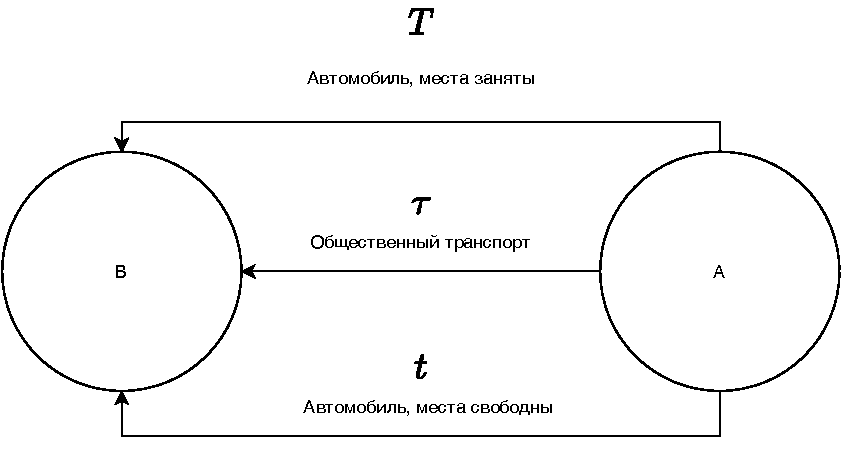
\includegraphics[scale=0.8]{img/task_scheme}


%\section{Рассуждения на тему задачи}

\section{Другие подходы к проблеме}
Транспортный поток как физическая материя, состоящая из молекул \cite[168]{lukanin}
\section{Варианты практического решения}
Ценовое регулирование
